% !TeX root = Bericht.tex
% !TeX spellcheck = de_DE
\section{Theory}
Light exhibits different phenomena when brought into contact with solid matter (E.g. absorption, scattering, diffraction). In this experiment we will make use of a special kind of diffraction, Bragg diffraction. This played a major role in uncovering the internal structure of crystal, exposing the position of their constituting atoms. 

\subsection{Bragg condition}
When shining light onto a crystal structure, the waves get partially reflected by the different lattice planes. In order to get constructive interference, the path difference between the different reflected light waves has to be an integer multiple of its wavelength $\lambda$. This is also known as the Bragg condition and is pictured in \autoref{fig:AOM} on the left.

\begin{figure}[H]
	\begin{subfigure}{.5\textwidth}
		\centering
		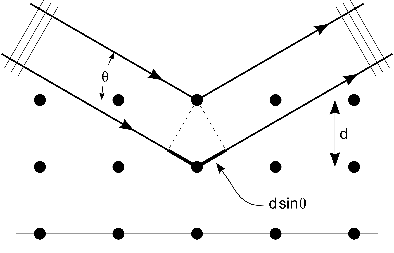
\includegraphics[width=.95\textwidth]{bragg}
	\end{subfigure}
	\begin{subfigure}{.5\textwidth}
		\centering
		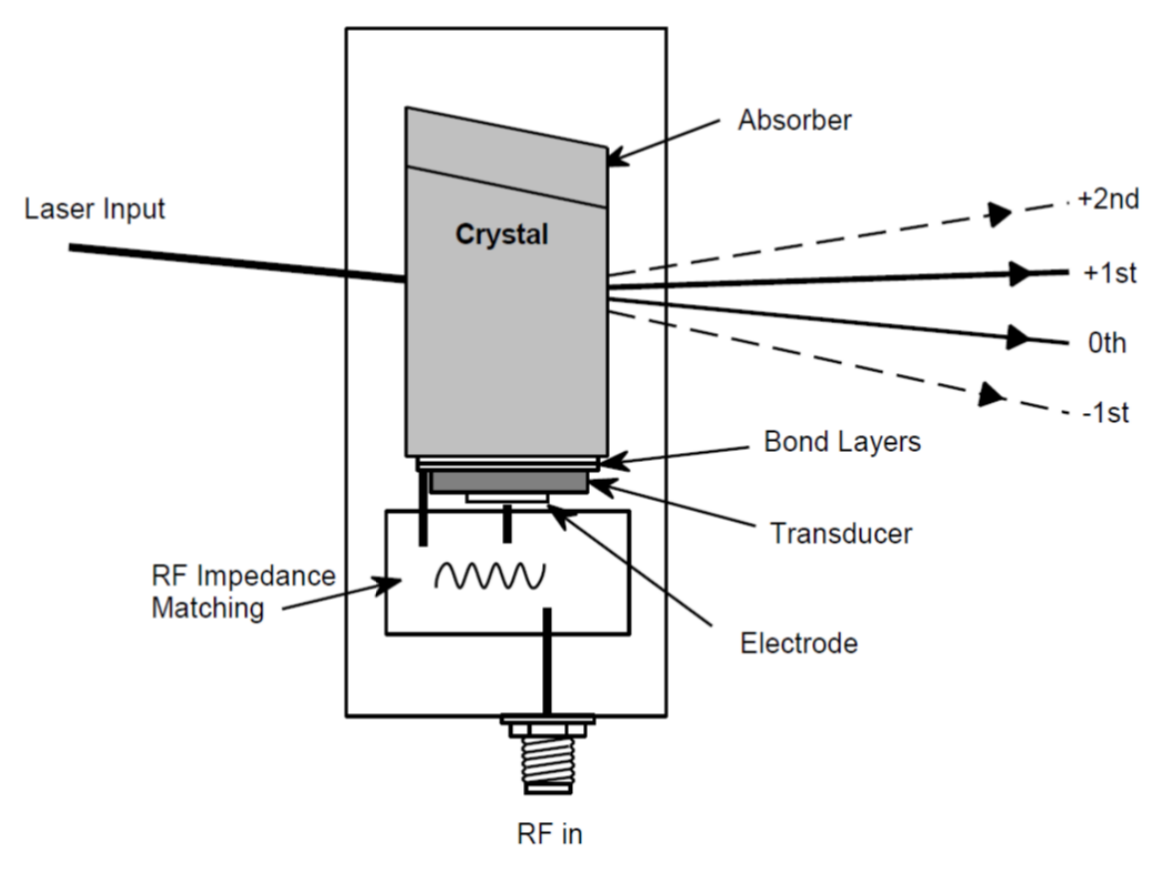
\includegraphics[width=.95\textwidth]{AOM}
	\end{subfigure}
	\caption{On the left side is the schematic sketch of the Bragg reflection  \autocite{bragg}. On the right is an overview of the working principle of an AOM. The RF signal gets coupled to the AOM via a piezo transducer. This creates density modulation inside the crystal, which divert the light beams intensity into higher diffraction orders \autocite{skript}.}
	\label{fig:AOM}
\end{figure}

Formally, the Bragg condition states that

\begin{equation}\label{eqn:bragg}
	n\lambda = 2d\sin(\theta),
\end{equation}

where \( d \) is the lattice plane spacing, \( n \) is an integer and \( \theta \) is the angle under which the light is shined on the crystal. 

\subsection{Acousto-optical modules}
\label{subsec:AOM}
In Acousto-optical modules (AOM) diffraction does not happen on fixed lattice planes. Instead, a change in refractive index is created by locally changing the density of the material. This can be done by inducing longitudinal waves (sound waves) into one side of the crystal and absorbing them on the other side to suppress standing waves. This creates periodic over- and under densities, which function like the static lattice planes. 

The sound waves are created by converting electric signals (from a function generator) into mechanical movement via a piezo element. An overview of an AOM's components is shown in \autoref{fig:AOM} on the right. 

As the AOM is not perfectly transparent for light waves, some losses occur due to absorption, which is defined as the ratio between the intensity before and after the AOM 
\[ IL = 1 - \frac{\P{out}}{\P{in}}. \]

Depending on the frequency \frf and the amplitude \( \P{RF} \) of the driving signal, more power is moved from the \nth{0} diffraction order (undisturbed transmission) to higher orders. For frequencies around the AOM's resonant frequency \(f_0 \sim 80 \unit{MHz} \) \autocite{AOM} most of the power gets diverted into the \nth{1} diffraction order. The efficiency \( \varepsilon = P_1/\P{out} \) is then defined as the ratio between the power in the \nth{1} order and the total power after the AOM. 

The efficiency depends on both \frf and \( \P{RF} \). Holding the frequency \frf constant one can derive that 

\begin{equation}\label{eqn:epsilon2}
	\varepsilon \sim \sin^2\left(\frac{\pi}{2} \sqrt{P}\right),
\end{equation}

with \( P = \P{RF}/\P{sat} \) the normalized RF power, where $\P{sat}$ describes the saturation power. A change in frequency can also be expressed in a change in bragg angle, which leads to the following relations:

\begin{equation}\label{eqn:epsilon}
	\varepsilon \sim \mathrm{sinc}^2\left(\frac{Q}{4}\Delta\right) 
	\quad\text{or}\quad 
	\varepsilon \sim \mathrm{sinc}^2\left(\frac{Q}{4} F \left(1-F\right)\right).
\end{equation}

Here \( \Delta = \delta/\theta_\mathrm{B} \) is the normalized angular error and \( F = f_\mathrm{RF}/f_0 \) is the frequency detuning from the resonant point (see \autocite{skript}). 

